\documentclass[10pt]{beamer}
\usetheme{jambro}

\title[]{Macroeconomia I - Demanda agregada}
\author[]{Paulo Victor da Fonseca}
\date{21 de março de 2023}

\hypersetup{
    colorlinks = true,
    urlcolor = teal,
    linkcolor = teal    
}
\usepackage[portuguese]{babel}
\usepackage{subfig}
\usepackage{emoji}

\begin{document}

\begin{frame}[plain]
    \titlepage{
        \begin{center}
            \begin{minipage}{0.8\textwidth}
                \centering
            \end{minipage}
        \end{center}}
\end{frame}

\begin{frame}{Sumário}
    \tableofcontents
\end{frame}

\section{Overview}
\begin{frame}{Overview}
    \begin{itemize}
        \item Final dos anos 2000s: famílias e firmas reduziram seus gastos e a economia global entrou em período de recessão\bigskip
         
        \item Atualmente, há um consenso entre economistas de que a queda dramática no PIB mundial em 2008-2009 - Crise Financeira Global (CFG) - foi um choque adverso de demanda agregada\bigskip
         
        \item Objetivo deste bloco: desenvolver modelo macro com o lado da \textcolor{purple}{demanda agregada} de um sistema econômico que envolve decisões de consumo de famílias, firmas e governo
    \end{itemize}
\end{frame}

\begin{frame}{Overview}
    \begin{itemize}
        \item Como veremos mais adiante, o lado da \textcolor{purple}{oferta agregada} envolve as atividades produtivas de uma economia\bigskip
         
        \item Grandes variações de demanda agregada - i.e., nos gastos da economia como um todo - como aconteceu em 2008/2009 são incomuns\bigskip
         
        \item Em períodos de maior normalidade, deslocamentos nas decisões de gastos agregados e no lado da oferta agregada da economia são as fontes de flutuações irregulares de recessões para booms que formam os \textcolor{purple}{ciclos econômicos}
    \end{itemize}
\end{frame}

\begin{frame}{Overview}
    \begin{itemize}
        \item Se um período de contração de gastos agregados é previsto, há discussões na imprensa acerca da necessidade de intervenção por parte do BC para mitigar a provável recessão via cortes nas taxas de juros\bigskip
         
        \item O BC abaixaria as taxas de juros com o objetivo de estimular os gastos agregados e, assim, auxiliar à economia a retomar estabilidade\bigskip
         
        \item De maneira similar, se espera-se um boom nos gastos agregados, o BC poderia mitigá-lo via aumentos na taxa básica de juros
    \end{itemize}
\end{frame}

\begin{frame}{Overview}
    \begin{itemize}
        \item Da mesma forma que a autoridade monetária, o governo central também precisa formular seus modelos acerca de como os padrões de gastos agregados provavelmente evoluem ao longo do tempo e como afetam o produto\bigskip
         
        \item Pois um período de recessão criará efeitos adversos sobre receitas arrecadadas via tributação e aumentar gastos com seguro-desemprego\bigskip
         
        \item Portanto, prever os padrões de gastos agregados é uma prioridade não só para agentes econômicos mas, também, para formuladores de política econômica - autoridades fiscal e monetária
    \end{itemize}
    
\end{frame}

\section{Demanda agregada e decisões de gastos}
\subsection{A composição do PIB}
\begin{frame}{Introdução}
    \begin{itemize}
        \item Foco desta seção: decisões de gastos e como influenciam o nível de atividade econômica\bigskip
         
        \item Por nível de atividade econômico estamos nos referindo a produto ou renda agregados\bigskip
         
        \item Quando o produto agregado varia, o nível de emprego também se altera\bigskip
         
        \item E.g., um aumento no nível de atividade econômica demanda um número maior de trabalhadores ou um aumento no número de horas trabalhadas\bigskip
         
        \item Além disso, a massa salarial aumenta e, com um número maior de vendas, os lucros totais também são mais elevados\bigskip
         
        \item Por isso que variações na atividade econômica podem ser interpretadas como mudanças tanto no produto quanto na renda
    \end{itemize}
\end{frame}

\begin{frame}{Introdução}
    \begin{itemize}
        \item Decisões de consumo são complexas\bigskip
         
        \item A compra de uma máquina por uma empresa, a decisão de ir a um restaurante por um consumidor e a aquisição de aviões pelo governo federal são decisões muito diferentes, que dependem de fatores diferentes\bigskip
         
        \item Para estudarmos a determinação da demanda por bens e serviços, faz sentido decompor o produto agregado do ponto de vista dos diversos tipos de bens e serviços produzidos e dos diversos tipos de compradores desses bens
    \end{itemize}
\end{frame}

\begin{frame}{Introdução}
    \begin{itemize}
        \item Além disso, para \textcolor{purple}{consumidores}, a decisão de consumo envolve tanto um \textcolor{blue}{componente estático} (o que comprar hoje dado a renda corrente e os preços dos bens e serviços disponíveis?) e um \textcolor{blue}{componente intertemporal} (como alocar consumo ao longo do tempo dadas as expectativas acerca de como a renda evolui ao longo do tempo?)\bigskip
         
        \item O processo decisório das firmas e governo também envolve um componente intertemporal\bigskip
         
        \item Decisões de aquisição de máquinas e equipamentos baseadas em um plano de negócios que inclui previsões acerca de como os custos e a demanda por seus produtos irão evoluir ao longo do tempo\bigskip
         
        \item O governo também deve prever as tendências demográficas quando faz planos de construção de novas escolas e hospitais
    \end{itemize}
\end{frame}

\begin{frame}{Introdução}
    \begin{itemize}
        \item As decisões destes agentes  que compõem o sistema econômico - firmas, famílias e governos - estão por trás do lado da demanda da economia\bigskip
         
        \item No entanto, a macroeconomia preocupa-se com a soma agregada das decisões de gastos destes grupos, e as consequências que suas decisões tem sobre os resultados agregados na economia como: taxas de inflação e de desemprego
    \end{itemize}
\end{frame}

\begin{frame}{Componentes do PIB}
    \begin{figure}
        \centering
        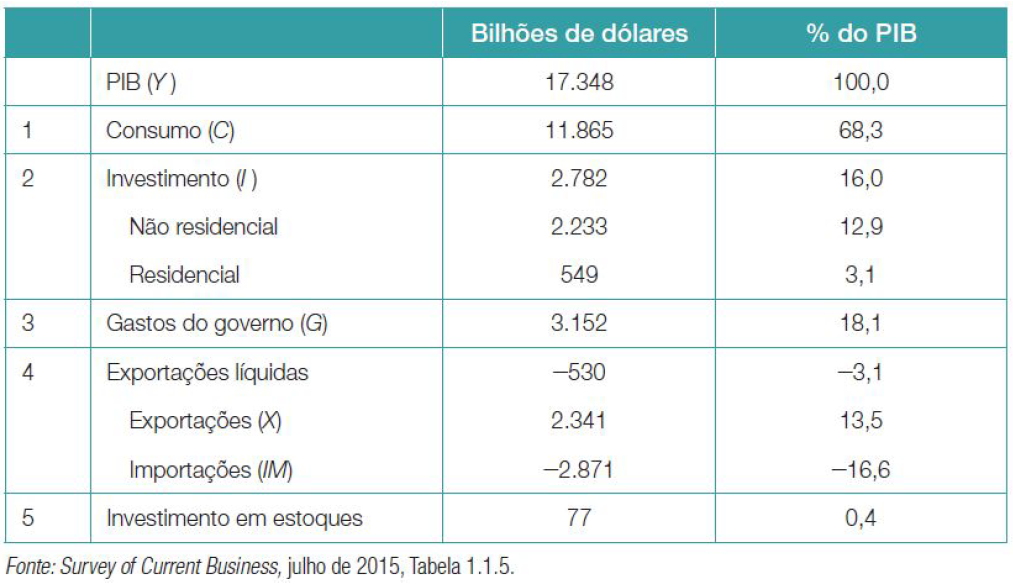
\includegraphics[width=0.8\textwidth]{./figures/aula5_fig1.PNG}
        \caption{Composição do PIB dos EUA, 2014. Fonte: Blanchard (2017).}
        \label{aula5_fig1}
    \end{figure}
\end{frame}

\begin{frame}{Componentes do PIB}
\begin{center}
\begin{table}
    \begin{tabular}{ |m{20em}|r|r|  }
 \hline
 \multicolumn{3}{|c|}{\textbf{{PIB sob a ótica da despesa}}} \\
 \hline
 \hline
 Componente do PIB & Valor total & \% do PIB \\
 \hline
\rowcolor{lightgray} \textcolor{blue}{PIB (Y)} & 7.004.141 & 100\% \\
 \hline
 \rowcolor{lightgray}
 Despesa de consumo final & 5.919.281 & 84,5\% \\
 \textcolor{blue}{Despesa de consumo das famílias (C)} & 4.423.548 & 63,2\% \\
Despesa de consumo das Instituições sem fins de lucro
          a serviço das famílias & 102.253 & 1,46\% \\ 
\textcolor{blue}{Despesa de consumo do governo (G)} & 1.393.480 & 19,9\% \\
\hline
\rowcolor{lightgray}
Formação bruta de capital & 1.057.278 & 15,1\% \\
\textcolor{blue}{Formação bruta de capital fixo (I)} & 1.057.409 & 15,1\% \\
Variação de estoque & \textcolor{red}{-131} & \textcolor{red}{-0,002\%} \\
\rowcolor{lightgray}
Saldo de balança comercial & 27.582 & 0,39\% \\
\textcolor{blue}{Exportação de bens e serviços (X)} & 1.025.056 & 14,63\% \\
\textcolor{blue}{Importação de bens e serviços (IM)} & \textcolor{red}{997.474} & \textcolor{red}{-14,24\%} \\
 \hline
\end{tabular}
\caption{Composição do PIB brasileiro, 2018. Fonte: IBGE, Diretoria de Pesquisas, Coordenação de Contas Nacionais.}
\end{table}
\end{center}
\end{frame}

\begin{frame}{Componentes do PIB}
    \begin{itemize}
        \item Consideraremos os seguintes componentes do PIB:\bigskip
        \begin{enumerate}
            \item \textcolor{blue}{Consumo (C):} bens e serviços adquiridos pelos consumidores - variam de alimentos a passagens aéreas, automóveis novos, etc. É o maior componente do PIB\medskip
            % 
            \item \textcolor{blue}{Investimento (I):} investimento (ou formação bruta de capital fixo) refere-se à aquisição de bens de capital novos. Note que a compra de ouro, de ações transacionadas na bolsa de valores ou outros ativos financeiros não estão contemplados - investimentos financeiros\medskip
            % 
            \item \textcolor{blue}{Gastos do governo (G):} bens e serviços adquiridos pelos governos federal, estadual e municipal. Esta variável não inclui as transferências do governo nem pagamentos de juros sobre a dívida pública
        \end{enumerate}
    \end{itemize}
\end{frame}

\begin{frame}{Componentes do PIB}
\begin{enumerate}
    
    \item[4.] \textcolor{blue}{Exportações (X):} compras de bens e serviços produzidos internamente no país por estrangeiros\medskip
    \item[5.] \textcolor{blue}{Importações (IM):} compras de bens e serviços estrangeiros por parte de consumidores, empresas e governo do país considerado\medskip
    \item[6.] \textcolor{blue}{Exportações líquidas (X-IM):} ou \textcolor{blue}{saldo da balança comercial} é a diferença entre exportações e importações. Se exportações excedem importações - \textbf{superávit comercial}. Caso contrário, um \textbf{déficit comercial}\medskip
    \item[7.] \textcolor{blue}{Investimento em estoques:} produção e vendas em um dado ano não precisam ser iguais. Alguns dos bens produzidos em um ano não são vendidos naquele ano, mas em anos posteriores. Alguns dos bens vendidos em um dado ano podem ter sido produzidos em anos anteriores. A diferença entre bens produzidos e bens vendidos em um dado ano é chamada de investimento em estoques
\end{enumerate}
\end{frame}

\subsection{Demanda agregada e política econômica}
\begin{frame}{Demanda agregada e política econômica}
    \begin{itemize}
        \item Dois dos principais instrumentos de política macroeconômica - políticas fiscal e monetária - influenciam diferentes elementos no lado da demanda agregada\bigskip
         
        \item Formuladores de política econômica preocupam-se com flutuações na demanda agregada pois afetam tanto o desemprego quanto a inflação\bigskip
         
        \item A \textcolor{purple}{política monetária} tem o objetivo de estabilizar a demanda agregada via alterações na taxa de juros (que afetam as decisões de investimento por parte das firmas e a aquisição de bens de consumo duráveis como novos carros e casas por parte das famílias)
    \end{itemize}
\end{frame}

\begin{frame}{Demanda agregada e política econômica}
    \begin{itemize}
        \item Aumento na taxa de juros leva a aumento nos custos de financeamento de novos projetos de investimento e projetos que seriam realizados a uma taxa de juros mais baixa seriam postergados ou cancelados\bigskip
         
        \item A política monetária também tem efeito indireto dado que a taxa de juros influencia os incentivos de poupar e, portanto, desloca as decisões de consumo ao longo do tempo\bigskip
         
        \item E.g., ao fazer com que os novos empréstimos tornem-se mais custosos e aumentar o retorno sobre a poupança, uma taxa de juros mais elevada irá encorajar as famílias a postergar o consumo presente
    \end{itemize}
\end{frame}

\begin{frame}{Demanda agregada e política econômica}
    \begin{itemize}
        \item Via variações nos gastos do governo em bens e serviços, a \textcolor{purple}{política fiscal} afeta a demanda agregada de maneira direta\bigskip
         
        \item Política fiscal também pode ser utilizada para influenciar a demanda agregada de maneira indireta, via efeitos sobre a renda das famílias e, portanto, suas decisões de consumo\bigskip
         
        \item É assim que variações nos impostos e transferências realizadas pela autoridade fiscal sob a forma de pensões, benefícios direcionados aos desempregados, etc. influenciam demanda agregada\bigskip
         
        \item \hlight{Nosso objetivo é desenvolver um modelo que explicite os mecanismos de transmissão com que as políticas fiscal e monetária afetam a economia, via decisões de gastos por parte das famílias, firmas e governo}
    \end{itemize}
\end{frame}

\subsection{Demanda agregada e ciclos econômicos: Fatos estilizados}
\begin{frame}{Participações no PIB}
    \begin{figure}
        \centering
        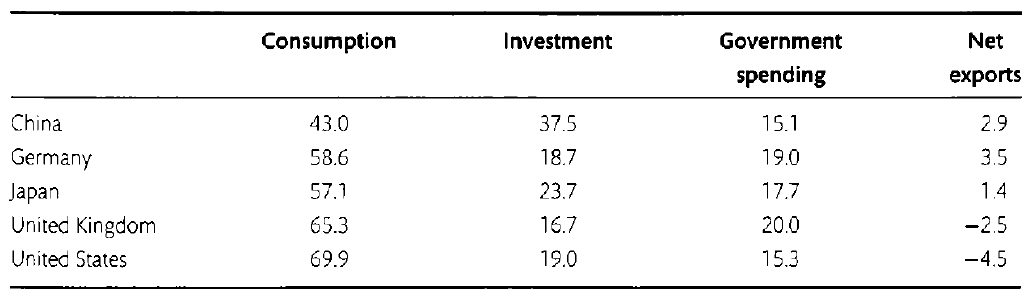
\includegraphics[width=\textwidth]{./figures/aula5_fig2.PNG}
        \caption{Componentes do PIB (\%), preços correntes, média 2000-2005. Fonte: Carlin e Soskice (2015).}
        \label{aula5_fig2}
    \end{figure}
\end{frame}

\begin{frame}{Participações no PIB}
    \begin{itemize}
        \item Composição média do PIB nas 5 principais economias industriais 2000-2005 evidencia que o consumo é o principal componente\bigskip
         
        \item A importância do consumo no PIB varia de 43\% na China a  $\approx 70\%$ nos EUA\bigskip
         
        \item Grande parte desta variação pode ser explicada pelas diferenças na contribuição do fator investimento\bigskip
         
        \item Uma proporção grande do PIB chinês é explicada pelos gastos privados com investimento, que deslocam os gastos com consumo
    \end{itemize}
\end{frame}

\begin{frame}{Participações no PIB}
    \begin{itemize}
        \item A figura também evidencia as variações entre países no que diz respeito às contribuições das exportações líquidas\bigskip
         
        \item Em média, entre 2000 e 2005, os EUA e o UK apresentaram déficits de conta corrente, enquanto os outros três países apresentaram um superávit de balança comercial, com exportações superando as importações
    \end{itemize}
\end{frame}

\begin{frame}{Participações no PIB}
    \begin{figure}
        \centering
        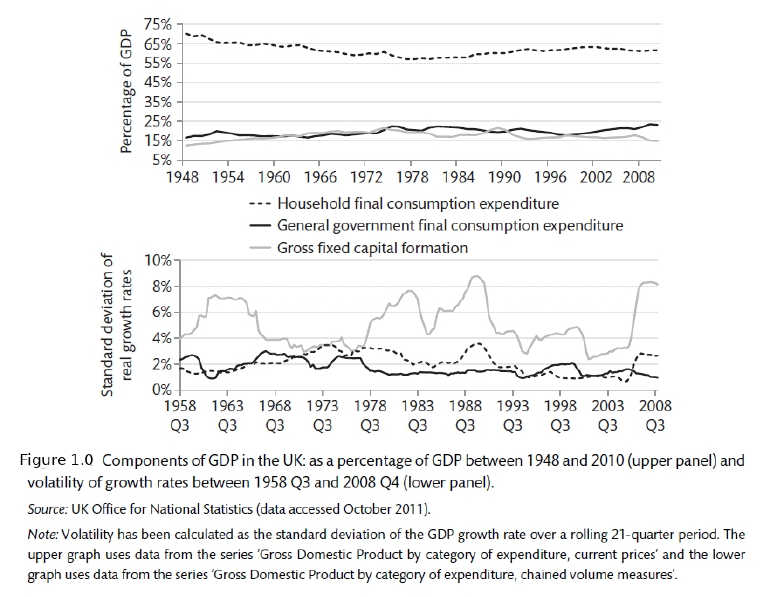
\includegraphics[width=0.55\textwidth]{./figures/aula5_fig3.PNG}
        \caption{Componentes do PIB e volatilidade: UK. Fonte: Carlin e Soskice (2015).}
        \label{aula5_fig3}
    \end{figure}
\end{frame}

\begin{frame}{Participações no PIB}
    \begin{itemize}
        \item Painel superior: evolução das participações do consumo, investimento e gastos do governo no PIB (UK - 1948 a 2010)\bigskip
         
        \item Painel inferior: volatilidade relativa das taxas de crescimento dos três componentes da DA\bigskip
         
        \item Investimento é muito mais volátil que o consumo e gastos do governo\bigskip
         
        \item Gastos com investimento dependem das expectativas de lucros pós-taxação e são muito dependentes do quão otimistas as firmas são\bigskip
         
        \item Além disso, decisões de investimento podem ser postergadas em períodos de recessão, consumo por parte das famílias e gastos do governo não podem ser tão facilmente postergados
    \end{itemize}
\end{frame}

\begin{frame}{Participações no PIB}
    \begin{itemize}
        \item \textcolor{purple}{Investimento é pró-cíclico}: elevado em períodos de booms e baixo em recessões\bigskip
         
        \item Apesar da participação relativa baixa no PIB, investimento é um fator determinante do ciclo econômico\bigskip
         
        \item Consumo mais elevado em termos de participação e menos volátil dado que hábitos de consumo das famílias são relativamente constantes\bigskip
         
        \item Mas como sua participação é elevada, pequenas variações no consumo podem ter efeitos consideráveis na economia como um todo\bigskip
         
        \item À medida que as flutuações adversas tornam-se mais extremas, temos o que chamamos de uma \textcolor{purple}{recessão econômica}\bigskip
         
        \item Definição popular de recessão: dois trimestres de crescimento negativo\bigskip
         
        \item No entanto, nem todas as recessões apresentam crescimento negativo. A definição é mais uma regra de bolso que uma regra estrita
    \end{itemize}
\end{frame}

\begin{frame}{Crescimento e ciclos econômicos}
    \begin{itemize}
        \item EUA: \href{https://www.nber.org}{NBER} responsável pela definição oficial de períodos de recessão
         
        \item Em 08/06/2020 o NBER reportou que a economia norte-americana entrou em um período de recessão. Este foi o anúncio mais rápido já feito:
        \begin{figure}
            \centering
            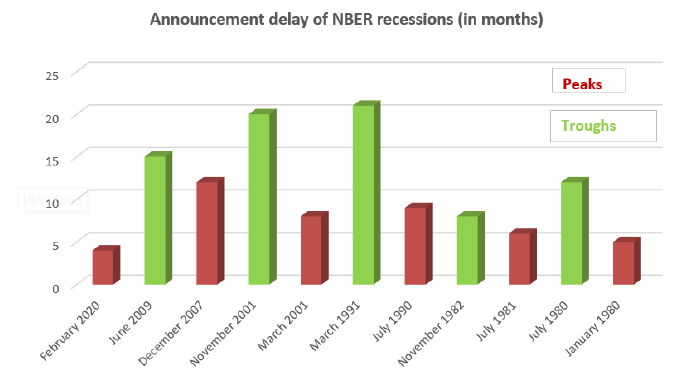
\includegraphics[width=0.65\textwidth]{./figures/aula5_fig4.PNG}
            \caption{Defasagem nos anúncios de recessão da economia americana (NBER). Fonte: \href{http://econbrowser.com/archives/2020/06/guest-contribution-a-severe-us-recession}{Econbrowser}.}
            \label{aula5_fig4}
        \end{figure}
    \end{itemize}
\end{frame}

\begin{frame}{Crescimento e ciclos econômicos}
    \begin{itemize}
        \item A recessão econômica gerada pela pandemia do COVID-19 e a CFG de 2007-2008 foram as duas maiores recessões registradas na história\bigskip
         
        \item Estes dois choques adversos aconteceram após um período que ficou conhecido como a \textcolor{purple}{Grande Moderação}, dada a relatividade estabilidade das economias desenvolvidas\bigskip
         
        \item O período da Grande Moderação pode ser observado na próxima figura, onde a janela rolante do desvio-padrão do PIB é registrada
    \end{itemize}    
\end{frame}

\begin{frame}{Crescimento e ciclos econômicos}
    \begin{figure}
        \centering
        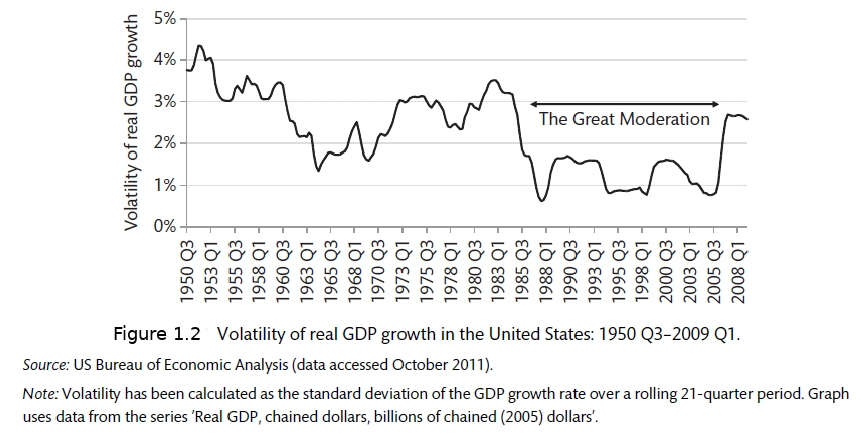
\includegraphics[width=0.85\textwidth]{./figures/aula5_fig5.PNG}
        \caption{Volatilidade do crescimento do PIB: EUA (1950-2009). Fonte: Carlin e Soskice (2015).}
        \label{aula5_fig5}
    \end{figure}
\end{frame}

\begin{frame}{Crescimento e ciclos econômicos}
    \begin{itemize}
        \item Alguns economistas acreditam que existe uma relação entre períodos de estabilidade e grandes perturbações ao sistema econômico\bigskip
         
        \item Antes da CFG, macroeconomistas acreditam que boas práticas na condução de políticas econômicas levaram a um período de grande estabilidade macroeconômica\bigskip
         
        \item Este período de estabilidade fez com que agentes econômicos ficassem mais complacentes, o que pode ter desencadeado um período de crise\bigskip
         
        \item Evidentemente, existem questionamentos a respeito do uso do PIB como uma variável de mensuração do bem-estar econômico - para maiores informações \href{https://www.khanacademy.org/economics-finance-domain/macroeconomics/macro-economic-indicators-and-the-business-cycle/macro-limitations-of-gdp/a/how-well-gdp-measures-the-well-being-of-society-cnx}{Khan academy}
    \end{itemize}
\end{frame}

\section{Demanda por bens e serviços}
\subsection{Introdução}
\begin{frame}{Introdução}
    \begin{itemize}
        \item Começaremos, agora, a formular um modelo que capture os elementos essenciais do sistema macroeconômico\bigskip
         
        \item Este modelo é conhecido como \textcolor{purple}{modelo de 3 equações} pois possui 3 elementos fundamentais:\bigskip
         
        \begin{enumerate}
            \item O lado da \hlight{demanda agregada}: curva IS\medskip
             
            \item O lado da \hlight{oferta agregada}: Curva de Phillips\medskip
             
            \item Comportamento do \hlight{formulador de política econômica}: regra de política monetária
        \end{enumerate}
    \end{itemize}
\end{frame}

\subsection{Demanda agregada e produto de equilíbrio}
\begin{frame}{Demanda agregada}
    \begin{itemize}
        \item Curva IS representa a demanda agregada\bigskip
         
        \item IS pois refere-se às decisões de investimentos planejados (I) e de poupança (S)\bigskip
         
        \item Formulada como uma simplificação da descrição do princípio de demanda efetiva de Keynes\bigskip
         
        \item A curva IS também é um dos componentes fundamentais do modelo IS/LM introduzido por John Hicks em 1937 e popularizado por Alvin Hansen nos EUA
    \end{itemize}
\end{frame}

\begin{frame}{Demanda agregada}
    \begin{itemize}
        \item A curva IS resume a forma com que o produto agregado é afetado por variações nas decisões de gastos de famílias, firmas e governo\bigskip
         
        \item E.g., quando firmas aumentam gastos com novos equipamentos, isso desencadeia um aumento produtivo no setor produtivo de bens de capital\bigskip
         
        \item Um número maior de indivíduos é empregado para produzir estes bens de capital adicionais e, à medida que gastam os salários recebidos, a demanda por bens de consumo também aumenta, levando a aumentos no emprego e produção nestes outros setores\bigskip
         
        \item Como resultado deste processo, a economia se deslocará para um nível mais elevado de produto e emprego
    \end{itemize}
\end{frame}

\begin{frame}{Demanda agregada}
    \begin{itemize}
    \item Veremos que em resposta à expansão inicial nos gastos, o produto se expandirá até o ponto em que a poupança adicional que os consumidores desejam fazer se iguale aos gastos adicionais com investimento\bigskip
     
    \item Neste ponto, o processo pelo qual o impacto inicial sobre a demanda agregada é multiplicado pela economia em rodadas subsequentes de emprego mais elevado, aumento nos gastos realizados por trabalhadores recém-admitidos, maior demanda por bens de consumo, etc., é completado
    \end{itemize}
\end{frame}

\begin{frame}{Demanda agregada}
    \begin{itemize}
        \item Focando nossas atenções no setor privado da economia, o nível de demanda agregada será determinado pela \textcolor{blue}{renda corrente} e pelos seguintes fatores:\bigskip
         
        \begin{enumerate}
            \item \textcolor{purple}{Expectativas a respeito do futuro}\medskip
            \begin{itemize}
                \item Planos de investimento das firmas dependem das expectativas com relação aos lucros futuros pós-taxação\medskip
                 
                \item Se firmas antecipam níveis mais elevados de utilização da capacidade, elas aumentarão seus investimentos em novas plantas/bens de capital\medskip
                 
                \item Famílias preferem ter uma trajetória suave de consumo, ao invés de flutuante\medskip
                 
                \item I.e., precisam poupar e tomar empréstimos de forma a distribuir consumo de maneira mais uniforme ao longo do tempo\medskip
                 
                \item Para tomar decisões acerca de poupança/empréstimos, precisam formar expectativas a respeito do crescimento futuro de sua renda
            \end{itemize}                        
        \end{enumerate}
    \end{itemize}
\end{frame}

\begin{frame}{Demanda agregada}
    \begin{itemize}
        \item A \textcolor{purple}{teoria do ciclo de vida} para a poupança se refere à poupança planejada levando em consideração o padrão de renda projetado de um indivíduo durante sua vida ativa e aposentadoria\bigskip
         
        \item Famílias revisarão para cima suas estimativas do quanto podem dispender  em cada período caso obtenham novas informações que façam com que esperem um crescimento maior de suas rendas\bigskip
         
        \item Decisões de dispêndio de firmas e famílias são tomadas em um cenário caracterizado por incerteza\bigskip
         
        \item E.g., um aumento na taxa de desemprego da economia pode sinalizar para as famílias que a incerteza a respeito de seus rendimentos futuros aumentou, o que levaria a um aumento na \textcolor{purple}{poupança precaucionária}
    \end{itemize}
\end{frame}

\begin{frame}{Demanda agregada}
    \begin{enumerate}
        
        \item[2.] \textcolor{purple}{Restrição de liquidez}\bigskip
         
        \begin{itemize}
            \item Pode emergir devido à dificuldade das instituições financeiras em avaliar credibilidade de famílias e firmas\medskip
             
            \item É impossível para bancos comerciais terem informação completa a respeito dos projetos e ações dos tomadores de empréstimo\medskip
             
            \item Neste caso, empréstimos para famílias e firmas de pequeno/médio porte podem ser restringidos por parte dos bancos\medskip
             
            \item Famílias e firmas que não podem tomar empréstimos em uma magnitude que desejam são chamados de \textcolor{purple}{restritos pela liquidez}\medskip
             
            \item Os problemas informacionais inerentes aos empréstimos bancários significam que o acesso ao crédito é, comumente, altamente dependente da quantidade de \textcolor{purple}{colateral} que o tomador de empréstimo possui, com o qual ele pode assegurar seus empréstimos
        \end{itemize}        
    \end{enumerate}
\end{frame}

\begin{frame}{Demanda agregada}
    \begin{itemize}
        \item A forma mais comum de colateral para famílias é o valor de seus imóveis\bigskip
         
        \item Isso significa que variações nos valores do colateral, que ocorre e.g. quando o preço dos imóveis varia, afetam o consumo e o investimento dado que restringem ou relaxam  as restrições de crédito
    \end{itemize}
\end{frame}

\begin{frame}{Demanda agregada}
    \begin{enumerate}        
    \setcounter{enumi}{2}
        \item \textcolor{purple}{Taxa de juros}\bigskip
         
        \begin{itemize}
            \item A taxa de juros pode afetar a demanda agregada por vários canais distintos - ver \textcolor{purple}{mecanismos de transmissão da política monetária} no site do \href{https://www.bcb.gov.br/controleinflacao/transmissaopoliticamonetaria}{Banco Central do Brasil}\medskip
             
            \item Quando a taxa de juros aumenta, famílias percebem um aumento nos valores das hipotecas\medskip
             
            \item Isso faz com que a demanda por novos imóveis seja reduzido e, além disso, reduz a demanda por móveis e outros bens de consumo duráveis\medskip
             
            \item Juros mais altos fazem com que as firmas restrinjam seus planos de gastos em novos equipamentos de capital e plantas industriais\medskip
             
            \item Famílias tendem a postergar consumo presente, dado que agora o retorno sobre poupança é mais elevado
        \end{itemize}
    \end{enumerate}
\end{frame}

\begin{frame}{Demanda agregada}
    \begin{itemize}
        \item No entanto, espera-se que famílias credoras e devedoras reajam de maneira distinta\bigskip
         
        \item Uma família credora perceberá um aumento de renda quando a taxa de juros se eleva e isso, por sua vez, leva a um aumento nos gastos via efeito-renda\bigskip
         
        \item Para famílias devedoras, o efeito é oposto\bigskip
         
        \item Normalmente, uma taxa de juros mais elevada está associada a uma demanda agregada mais baixa
    \end{itemize}
\end{frame}

\begin{frame}{Demanda agregada e produto de equilíbrio}
    \begin{itemize}
        \item A \textcolor{blue}{demanda agregada} $Z$ é a quantidade total de bens demandados na economia\bigskip
         
        \item Usando a composição do PIB que acabamos de ver, podemos escrever a seguinte identidade:
        \begin{equation}
            Z \equiv C + I + G + X - IM.
        \end{equation}
         
        \item O produto está em seu nível de equilíbrio quando a quantidade produzida for igual à quantidade demandada:
        \begin{equation}
            Y = Z = C + I + G + X - IM.
        \end{equation}
         
        \item Quando a demanda agregada não for igual ao produto, há o investimento ou desinvestimento não planejado em estoques:
        \begin{equation}
            IU = Y - Z,
        \end{equation}
        em que $IU$ representa os acréscimos não planejados ao estoque.
    \end{itemize}
\end{frame}

\begin{frame}{Hipóteses simplificadoras}
    \begin{itemize}
        \item Todas as empresas produzem o mesmo bem, que pode ser utilizado pelos consumidores para consumo, pelas empresas para investimento ou pelo governo. Podemos, assim, examinar apenas um mercado - o de um único bem - e pensar no que determina a oferta e demanda nesse mercado\bigskip
         
        \item Empresas estão dispostas a ofertar qualquer montante desse bem a um dado preço, $P$. Esta hipótese permite que nos concentremos no papel desempenhado pela demanda na determinação do produto. Hipótese válida apenas para o curto prazo\bigskip
         
        \item Economia não transaciona com o resto do mundo (economia fechada). Portanto $X - IM = 0$ e:
        \begin{equation}
        Z \equiv C + I + G.
        \end{equation}
    \end{itemize}
\end{frame}

\subsection{Consumo}
\begin{frame}{Função consumo}
    \begin{itemize}
        \item As decisões de consumo dependem de muitos fatores\bigskip
         
        \item O principal deles é a renda ou, mais precisamente, a \textcolor{blue}{renda disponível ($Y_D$)}, a renda que resta depois que os consumidores receberam transferências do governo e pagaram seus impostos\bigskip
         
        \item A relação entre consumo e renda disponível é descrita pela \textcolor{blue}{função consumo} que nos diz que quando a renda disponível sobe (cai), as pessoas compram mais (menos) bens:
        \begin{equation}
            C = C(Y_d), \qquad C'(Y_D) > 0.
        \end{equation}
         
        \item É razoável supor que a relação entre consumo e renda disponível seja linear:
        \begin{equation}
            C = c_0 + c_1Y_D, \qquad c_0>0 \quad \text{e } 0<c_1<1.
            \label{consumo}
        \end{equation}
    \end{itemize}
\end{frame}

\begin{frame}{Relação entre consumo e renda disponível}
    \begin{figure}
        \centering
        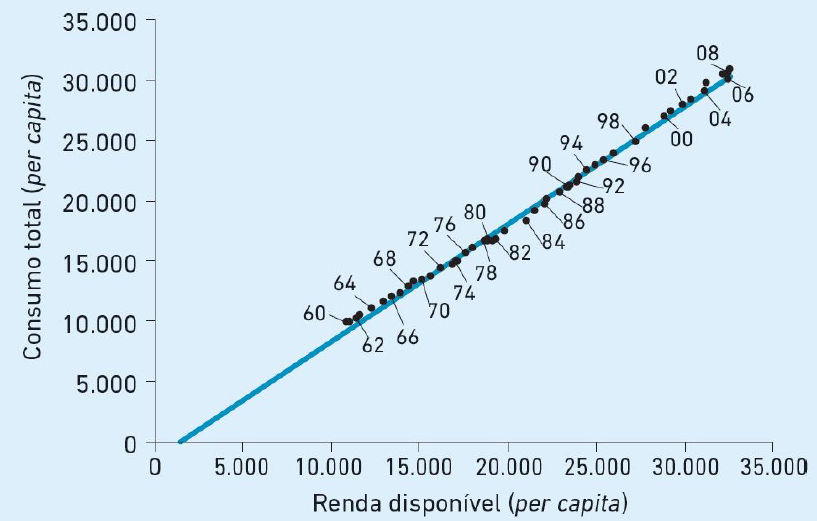
\includegraphics[width=0.7\textwidth]{./figures/aula5_fig6.PNG}
        \caption{Relação entre consumo e renda disponível - EUA 1960 a 2008. Fonte: Dornbusch et al. (2013)}
        \label{aula5_fig6}
    \end{figure}
\end{frame}

\begin{frame}{Relação entre consumo e renda disponível}
\begin{itemize}
    \item A figura anterior plota os dados anuais de consumo \emph{per capita} e da renda pessoal disponível \emph{per capita} desde 1960\bigskip

    \item A  relação linear entre consumo e renda disponível da equação (\ref{consumo}) é uma boa descrição inicial    
    
\end{itemize}
\end{frame}

\begin{frame}{Função consumo}
    \begin{itemize}
        \item A relação entre consumo e renda disponível é, então, caracterizada por dois parâmetros $c_0$ e $c_1$\bigskip
         
        \item O parâmetro $c_0$, o intercepto da função, pode ser interpretada das seguintes formas:\bigskip
         
        \begin{itemize}
            \item Nível de consumo quando a renda disponível é nula. Uma restrição natural é que se a renda corrente for zero, o consumo ainda será positivo: com ou sem renda, as pessoas precisam comer! Como isso é possível? As famílias despoupam, i.e., consomem vendendo alguns de seus ativos ou contraindo algum empréstimo\medskip
             
            \item Alterações em $c_0$ refletem mudanças no consumo para um dado nível de renda disponível. Aumentos (diminuições) em $c_0$ refletem um aumento (diminuição) no consumo para uma dada renda. Há muitas razões pelas quais as pessoas podem decidir consumir mais ou menos, dado seu rendimento disponível - e.g., achar mais fácil ou difícil tomar empréstimos, ou tornar-se mais ou menos otimista com relação ao futuro
        \end{itemize}
    \end{itemize}
\end{frame}

\begin{frame}{Função consumo}
\begin{itemize}
    \item O parâmetro $c_1$, por sua vez, é chamado de \textcolor{blue}{propensão marginal a consumir}. Mostra o efeito de uma unidade monetária adicional de renda disponível sobre o consumo\bigskip
     
    \item Uma restrição natural é que $c_1$ seja positivo - aumento de renda disponível leva a aumento do consumo. Além disso, $c_1$ é menor que 1. As pessoas provavelmente consomem apenas uma parte de qualquer aumento da renda disponível e poupam o restante
\end{itemize}
\end{frame}

\begin{frame}{Função consumo}
    \begin{figure}
        \centering
        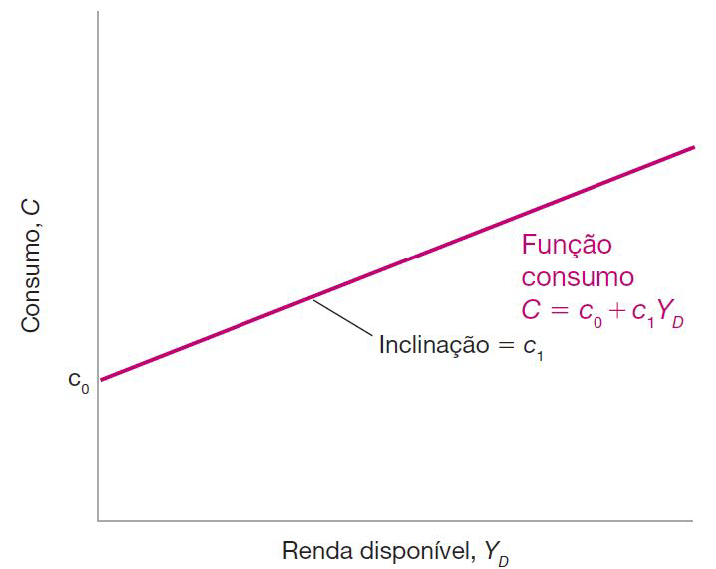
\includegraphics[width=0.55\textwidth]{./figures/aula5_fig7.PNG}
        \caption{Função consumo. Fonte: Blanchard (2017).}
        \label{aula5_fig7}
    \end{figure}
\end{frame}

\begin{frame}{Renda disponível}
    \begin{itemize}
        \item A renda disponível $Y_D$ é dada por:
        \begin{equation}
            Y_D \equiv Y - T,
        \end{equation}
        onde $Y$ é a renda e $T$ os impostos pagos menos as transferências do governo recebidas pelos consumidores\bigskip
         
        \item Portanto, a função consumo pode ser reescrita como:
        \begin{equation}
            C = c_0 + c_1(Y-T).
        \end{equation}
         
        \item Uma renda mais elevada aumenta o consumo, embora em uma proporção menor do que um para um\bigskip
         
        \item Impostos mais altos retraem o consumo, em proporção menor do que um para um
    \end{itemize}
\end{frame}

\subsection{Investimento}
\begin{frame}{Investimento}
    \begin{itemize}
        \item Inicialmente vamos tratar o nível de investimento como uma variável exógena e, portanto:
        \begin{equation}
            I = \bar{I}.
        \end{equation}
         
        \item Esta hipótese não é inócua, implica que mudanças na produção não impactam decisões de investimento\bigskip
         
        \item Mais tarde na disciplina relaxaremos esta hipótese
    \end{itemize}
\end{frame}

\subsection{Gastos do governo}
\begin{frame}{Gastos do governo}
    \begin{itemize}
        \item Terceiro componente da DA: gastos do governo $G$\bigskip
         
        \item As variáveis $T$ e $G$ descrevem a \textbf{política fiscal} do governo\bigskip
         
        \item Assumiremos que $T$ e $G$ são variáveis exógenas ao modelo. Nossa hipótese de exogeneidade pode ser explicada pelos seguintes motivos:\bigskip
         
        \begin{enumerate}
            \item Governos não se comportam de maneira tão sistemática como consumidores ou empresas - não há regras confiáveis que possamos adotar para descrever $G$ e $T$ que sejam análogas à regra de consumo que vimos anteriormente\medskip
             
            \item Macroeconomistas estão interessados nas implicações de decisões alternativas de política fiscal - gastos e tributação.
        \end{enumerate}
    \end{itemize}
\end{frame}

\section{Determinação do produto de equilíbrio}
\begin{frame}{Determinação do produto de equilíbrio}
    \begin{itemize}
        \item Em uma economia fechada, a demanda agregada pro bens e serviços é dada por:
        \[
        Z \equiv C + I + G.
        \]
         
        \item Portanto:
        \begin{equation}
            Z = c_0 + c_1(Y-T) + \bar{I} + G.
        \end{equation}
         
        \item Equilíbrio no mercado de bens e serviços requer que produção e demanda se igualem (investimento em estoques é sempre igual a zero). Portanto $Y = Z$ e:
        \begin{equation}
            Y = c_0 + c_1(Y-T) + \bar{I} + G.
        \end{equation}
         
        \item Em equilíbrio, a produção $Y$ é igual à demanda agregada. A demanda, por sua vez, depende da renda, $Y$, que é igual à produção (pela condição de equilíbrio).
    \end{itemize}
\end{frame}

\subsection{Solução do modelo}
\begin{frame}{Solução do modelo}
    \begin{itemize}
        \item Temos, portanto, que a renda de equilíbrio será dada por:
        \begin{equation}
            Y = \frac{1}{1-c_1}[c_0 + \bar{I} + G - c_1T].
        \end{equation}
         
        \item O termo $[c_0 + \bar{I} + G - c_1T]$ é a parte da demanda por bens e serviços que não depende do produto - \hlight{gasto autônomo}\bigskip
         
        \item O termo $1/(1-c_1)$ é um número maior que 1, dado que $0<c_1<1$. Por este motivo, esse número que multiplica o gasto autônomo é chamado de \hlight{multiplicador}. Quanto mais próximo $c_1$ estiver de 1, maior será o multiplicador
    \end{itemize}
\end{frame}

\subsection{Gasto autônomo}
\begin{frame}{Gasto autônomo}
    \begin{itemize}
        \item Não podemos, com certeza, determinar se o gasto autônomo é positivo. Mas é bem provável que seja\bigskip
         
        \item Os dois primeiros termos, $c_0$ e $\bar{I}$ são positivos. Mas o que podemos dizer acerca de $G-c_1T$?\bigskip
         
        \item Se o governo adotar um \textbf{orçamento equilibrado}, ou seja $T = G$, então, $G-c_1T$ será positivo e assim também será o gasto autônomo\bigskip
         
        \item Apenas se o governo tivesse um superávit orçamentário muito grande - impostos muito maiores que os gastos - é que o gasto autônomo poderia ser negativo\bigskip
         
        \item Podemos, seguramente, ignorar este caso
    \end{itemize}
\end{frame}

\subsection{Multiplicador}
\begin{frame}{Multiplicador}
    \begin{itemize}
        \item Em equilíbrio, a renda é igual à demanda agregada\bigskip
         
        \item Em quanto um aumento de $\$1$ no gasto autônomo eleva o nível de equilíbrio da renda?\bigskip
         
        \item Intuitivamente podemos dizer que um aumento de uma unidade monetária na demanda ou no gasto autônomo deve aumentar a renda de equilíbrio também em \$1\bigskip
         
        \item Vimos que:
        \[
        Y = \frac{1}{1-c_1}[c_0 + \bar{I} + G - c_1T].
        \]
         
        \item Ou seja, o produto aumentará em mais de \$1 devido ao efeito multiplicador\bigskip
         
        \item E.g., se $c_1 = 0,6$, o multiplicador é $1/(1-0,6) = 2,5$, de modo que o produto aumenta em \$2,5.
    \end{itemize}
\end{frame}

\begin{frame}{Multiplicador}
    \begin{itemize}
        \item De onde vem esse efeito multiplicador?\bigskip
         
        \item Um aumento no gasto autônomo aumenta a demanda\bigskip
         
        \item Um aumento da demanda, por sua vez, leva a um aumento da produção\bigskip
         
        \item O aumento da produção leva a um aumento equivalente da renda (lembre-se de que as duas são idênticas)\bigskip
         
        \item O aumento da renda aumenta o consumo, o que aumenta a demanda, e assim por diante
    \end{itemize}
\end{frame}

\begin{frame}{Representação gráfica}
    \begin{itemize}
        \item Renda e produção são sempre iguais, então, graficamente, a relação entre ambas é a reta de 45º (inclinação igual a 1)\bigskip
         
        \item E a demanda como função da renda é dada por:
        \[
        Z = (c_0 + \bar{I} + G - c_1T) + c_1Y
        \]
         
        \item A demanda depende do gasto autônomo e da renda, por meio do seu efeito sobre o consumo\bigskip
         
        \item O intercepto corresponde ao gasto autônomo e a inclinação é a propensão marginal a consumir $c_1 < 1$\bigskip
         
        \item Em equilíbrio, a produção é igual à demanda - o produto de equilíbrio é dado pela interseção da reta de 45º com a função demanda
    \end{itemize}
\end{frame}

\begin{frame}{Representação gráfica}
    \begin{figure}
        \centering
        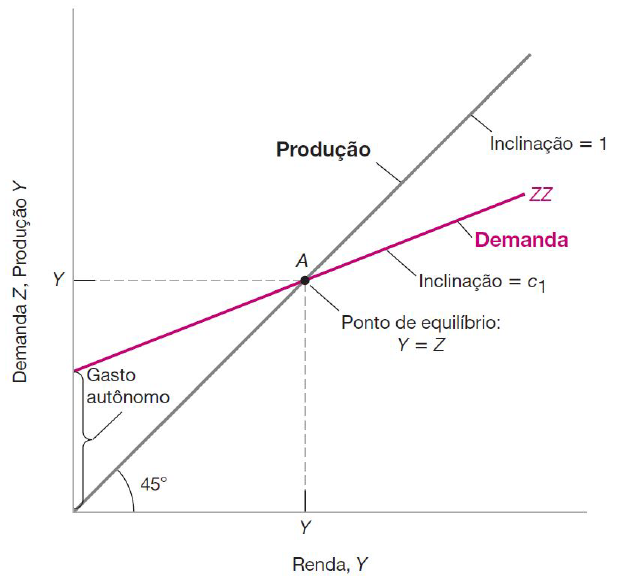
\includegraphics[width=0.5\textwidth]{./figures/aula5_fig8.PNG}
        \caption{Equilíbrio no mercado de bens. Fonte: Blanchard (2017).}
        \label{fig4}
    \end{figure}
\end{frame}

\begin{frame}{Representação gráfica: efeitos de um aumento no gasto autônomo}
\begin{figure}
    \centering
    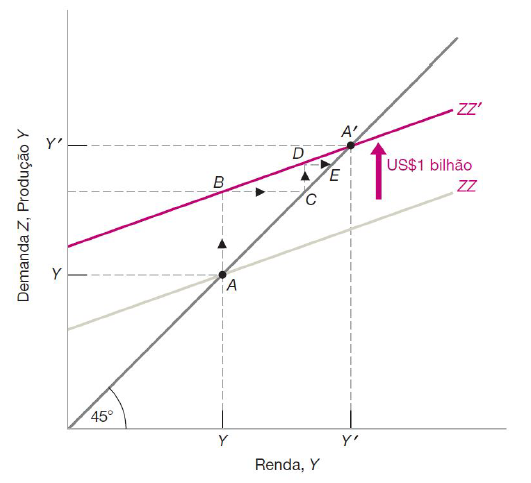
\includegraphics[width=0.5\textwidth]{./figures/aula5_fig9.PNG}
    \caption{Efeitos de um aumento do gasto autônomo sobre o produto de equilíbrio. Fonte: Blanchard (2017).}
    \label{fig5}
\end{figure}
\end{frame}

\begin{frame}{Representação gráfica: efeitos de um aumento no gasto autônomo}
    \begin{itemize}
        \item Suponha economia em equilíbrio inicial dado pelo ponto $A$ com produção igual a $Y$\bigskip
         
        \item Suponha que consumo autônomo $c_0$ aumente em \$1 bilhão\bigskip
         
        \item No nível inicial de renda, consumidores aumentam seu consumo em \$ 1 bilhão\bigskip
         
        \item Aumento de consumo desloca a curva de demanda de $ZZ$ para $ZZ'$ em \$ 1 bilhão\bigskip
         
        \item No nível inicial de renda $Y$, temos um excesso de demanda no ponto $B$\bigskip
         
        \item Para satisfazer nível mais alto de demanda, firmas aumentam produção em \$ 1 bilhão\bigskip
         
        \item Esse aumento de produção implica que a renda aumenta em \$ 1 bilhão, já que renda é igual a produção, logo, a economia se move para o ponto $C$
    \end{itemize}
\end{frame}

\begin{frame}{Representação gráfica: efeitos de um aumento no gasto autônomo}
\begin{itemize}
    \item Aumento de renda leva a aumento adicional da demanda de $\$ c_1$ bilhão, levando economia para o ponto $D$\bigskip
     
    \item Ponto $D$ leva a um nível de produção e renda mais altos em $\$c_1$ bilhão - ponto $E$\bigskip
     
    \item Este aumento de $c_1$ bilhão na renda leva a um aumento de $\$c_1^2$ bilhão na demanda, e assim por diante\bigskip
     
    \item Seguindo a lógica, o aumento total da produção após $n+1$ rodadas é igual a \$ 1 bilhão vezes a soma:
    \[
    1 + c_1 + c_1^2 + \dots + c_1^n.
    \]
     
    \item Essa soma é uma progressão geométrica e, como $c_1$ é menor que 1, o limite desta progressão é dado por $1/(1-c_1)$, que é exatamente o valor do multiplicador\bigskip
     
    \item Portanto, o aumento final do produto é igual a $\$\frac{1}{1-c_1}$ bilhão
\end{itemize}
\end{frame}

\begin{frame}{Exercício}
    \begin{itemize}
        \item Vimos a relação entre renda disponível e consumo para a economia norte-americana para o período 1960-2008\bigskip
         
        \item A função consumo estimada, neste caso, nos diz que a propensão marginal a consumir é $c_1 = 0,97$\bigskip
         
        \item Partindo de uma condição inicial de equilíbrio, suponha que os gastos do governo nos EUA aumentem em \$ 1 bilhão\bigskip
         
        \item De acordo com nosso modelo, qual será o efeito deste aumento sobre o produto de equilíbrio?
    \end{itemize}
\end{frame}

\begin{frame}{Exercício}
    Suponha que a economia seja caracterizada pelas seguintes equações comportamentais:
    \begin{eqnarray}
    C &=& 160 + 0,6Y_D, \nonumber \\
    I &=& 150, \nonumber \\
    G &=& 150, \nonumber \\
    T &=& 100. \nonumber
    \end{eqnarray}
    Resolva para as seguintes variáveis:
    \begin{enumerate}
        \item O PIB de equilíbrio ($Y_D$).
         
        \item A renda disponível ($Y_D$).
         
        \item Os gastos de consumo ($C$).
    \end{enumerate}
\end{frame}

\begin{frame}{\emoji{books} Bibliografia}
    \begin{itemize}
        \item BLANCHARD, O. Macroeconomia. 7.ed. São Paulo: Pearson Education do Brasil, 2017\medskip
        \item CARLIN, W.; SOSKICE, D. Macroeconomics: Institutions, instability, and the financial system. Oxford, UK: Oxford University Press, 2015\medskip
        \item DORNBUSCH, R.; FISCHER, S.; STARTZ, R. Macroeconomia. 11.ed. Porto Alegre: AMGH, 2013. Disponível em: \href{https://app.minhabiblioteca.com.br/books/9788580551853}{app.minhabiblioteca.com.br/books/9788580551853}\medskip
        \item KEYNES, J.M. \emph{A teoria geral do emprego, do juro e da moeda}. São Paulo: Atlas, 1992. (Data do original em inglês: 1936)\medskip        
    \end{itemize}
\end{frame}
\end{document}